\documentclass[10pt]{article}
\usepackage[T1]{fontenc}
\usepackage{mathptmx}
\usepackage[margin=1in]{geometry}
\usepackage{setspace}
\usepackage[table]{xcolor}
\usepackage{booktabs}
\usepackage{graphicx}
\usepackage[section]{placeins}
\usepackage{caption}
\captionsetup{font=small}
\setstretch{1.5}

\begin{document}

\noindent\textbf{Problem Set 1b: BHARs and Calendar-Time Portfolios after Stock Splits}

\medskip
\noindent\textbf{Approach.} Daily returns are compounded into calendar months (empty stock-days inside a stock's history, 91 in total, are filled with \texttt{mkt\_ret}). An event's window is months $+1$ to $+12$ after the ex-date month; data end in December 2025. Predictions (Table~\ref{tab:pred}) were written before any calculation. All numbers come from \texttt{ps1b.py}; checks are in the Appendix.

\medskip
\noindent\textbf{Q1 (event panel).} There are 232 events. Two have ex-dates in December 2025 and no window month, so 230 events give 2,681 event-month rows. Nineteen events (ex-dates in 2025) are cut short by the data end and 4 by the stock ceasing to trade (proceeds go to \texttt{mkt\_ret}; none of the 4 overlaps with the data-end group); 209 are complete (Table~\ref{tab:q1}, \ref{tab:q1b}).

\medskip
\noindent\textbf{Q2 (BHAR vs.\ market).} 213 events have a 12-month BHAR (Table~\ref{tab:bhar}, Figure~\ref{fig:bhar}). The mean is 0.74\% (median 1.53\%), s.e.\ 2.44\%, $t=0.30$ ($p=0.76$): not significant. The distribution is wide (sd 35.7\%; 10th/25th/75th/90th percentiles $-43.3$/$-21.6$/$18.6$/$44.1$\%) and mildly right-skewed ($\hat\gamma=0.41$). With this s.e., a mean BHAR must exceed 4.8\% to be significant at 5\%, and the true mean must be about 6.9\% to be detected with 80\% power: the test cannot rule out abnormal returns of a few percent a year.

\medskip
\noindent\textbf{Q3 (benchmark).} Using month-0 market cap (median \$5.3bn; 14\% of events in NYSE decile 1, 21\% in decile 10; Figure~\ref{fig:size}, Table~\ref{tab:decile}) and French's value-weighted decile returns, the mean BHAR rises to 3.06\% ($t=1.28$). The paired change of $+2.33$ pp (s.e.\ 0.49, $t=4.76$) is highly significant, but the conclusion is the same: the mean BHAR is not significantly different from zero under either benchmark. The benchmark matters because the value-weighted market is dominated by mega-caps: its average 12-month return over the windows (9.8\%) exceeds that of the average size-matched benchmark (7.5\%), since many splitters are small or mid-caps.

\medskip
\noindent\textbf{Q4 (skewness).} $t_{SA}=0.31$ versus $t=0.30$ (decile benchmark: 1.30 versus 1.28). The difference is negligible because skewness is modest and $S=\overline{\mathrm{BHAR}}/s$ is only 0.02, so the correction $\sqrt n(\hat\gamma S^2/3+\hat\gamma/6n)\approx 0.005$. In general, with positively skewed BHARs the sample mean and sample standard deviation are positively correlated, so the sampling distribution of $t$ is negatively skewed: the conventional test rejects too often in the lower tail and too rarely in the upper tail, i.e., it understates evidence of positive (and overstates evidence of negative) abnormal returns. The skewness-adjusted statistic corrects this, and the effect is immaterial here.

\medskip
\noindent\textbf{Q5 (calendar-time portfolio).} In each calendar month I hold every stock that is in months $+1$ to $+12$ of a split window, equally weighted, and a stock with overlapping splits is held once (8 duplicated stock-months removed, from 2,675 to 2,667). The portfolio spans 143 months (Feb 2014--Dec 2025, none empty) and holds 18.7 stocks on average (minimum 4, maximum 41). Twenty-two months hold fewer than 10 stocks, all between 2014 and Oct 2023; they are kept in the sample, so those months are noisy but get the same weight as the others (Table~\ref{tab:q5}, Figure~\ref{fig:port}). Weights sum to one in every month, and the monthly return has mean 0.94\% and sd 5.6\%.

\medskip
\noindent\textbf{Q6 (factor regressions).} The equal-weighted portfolio's raw mean excess return is 0.80\% per month (Newey-West $t=2.27$), but this is market risk: the CAPM alpha is $-0.32$\% ($t_{NW}=-1.52$, $t_{OLS}=-1.29$) with $\beta=1.10$, and alpha is $-0.12$\% ($-0.51$) with three factors, $-0.12$\% ($-0.53$) adding momentum, and $-0.11$\% ($-0.48$) in the five-factor model (Table~\ref{tab:q6}, Figure~\ref{fig:alpha}). Alpha rises by 0.20 pp from CAPM to three factors for two reasons (Table~\ref{tab:q6c}): the market loading falls to 1.00 (+0.10 pp) and the SMB loading is 0.51 ($t_{NW}=7.9$) while SMB earned $-0.22$\% per month in this sample (+0.11 pp). Together these remove about 60\% of the CAPM underperformance: splitters are small/mid-cap stocks that lagged in this period, and they carry a market beta close to one once size is controlled. HML ($-0.09$), momentum (0.01), RMW and CMA are insignificant. Newey-West standard errors for alpha are \emph{smaller} than OLS ones in models (1)--(2) (0.35 vs.\ 0.47; 0.21 vs.\ 0.25) and about equal afterwards (0.235 vs.\ 0.23), contrary to my prediction; conclusions do not depend on this choice (Table~\ref{tab:q6b}).

\medskip
\noindent\textbf{Q7 (comparison).} Both methods agree on the statistical conclusion: no significant abnormal return after splits (BHAR $+0.7$\%, $t=0.3$; CAPM alpha $-3.9$\% per year, $t=-1.5$; three-factor alpha $-1.4$\%, $t=-0.5$). The signs differ for CAPM because the two measures are not the same object (Table~\ref{tab:q7}, Figure~\ref{fig:bridge}): (i) the provided \texttt{mkt\_ret} compounds to 282\% over 2014--2025 against 342\% for French's market ($\approx$1.4 pp per year lower), so BHAR against French's market is $-0.6$\%; (ii) BHAR weights every event-month equally ($+0.9$\% per year, arithmetic) whereas calendar-time weights every calendar month equally, giving much weight to the early months held by only 4--10 stocks ($-1.35$\% against \texttt{mkt\_ret}); (iii) the CAPM penalises beta of 1.10 in a market that earned about 12\% per year (about $-1.2$ pp), while BHAR implicitly assumes beta 1; (iv) the calendar-time portfolio includes the truncated windows of the 2025 splits and is rebalanced monthly, while BHAR compounds buy-and-hold. Three-factor alphas are close to zero because the beta and size loadings absorb most of the CAPM underperformance.

\medskip
\noindent\textbf{Q8 (weighting).} Weighting does not change the conclusion (Table~\ref{tab:q8}, Figure~\ref{fig:weight}). Weighting months by the number of stocks held (WLS) gives CAPM alpha $-0.18$\% ($t=-0.81$) and three-factor alpha $+0.04$\% ($0.15$); the value-weighted portfolio gives $-0.07$\% ($-0.16$) and $-0.15$\% ($-0.41$). The value-weighted portfolio is extremely concentrated (the largest stock averages 50\% of the weight; effective number of stocks 3.7), so it is a mega-cap growth portfolio: $\beta=1.26$, HML $-0.75$, SMB $\approx 0$ (Table~\ref{tab:q8b}). Its CAPM alpha is closer to zero than the equal-weighted one because it lacks the small-cap tilt (SMB $\approx 0$) that hurt the equal-weighted portfolio; once three factors are included, all three alphas lie within $\pm0.15$ pp per month with $|t|<0.6$. Weighting changes the loadings, not the (insignificant) alpha.

\clearpage
\section*{Tables and Figures}

\begin{table}[!htbp]
\caption{Pre-analysis predictions (written before any calculation), with the outcome in the last column.}
\label{tab:pred}
\begin{tabular}{p{4.0cm}p{3.6cm}p{4.2cm}p{3.2cm}}
\toprule
Question & Prediction & Why? & Outcome \\
\midrule
Mean 12-month BHAR & About zero (slightly positive), statistically insignificant & Splitters follow price run-ups, but long-run abnormal returns are small and BHARs are very noisy (sd about 35--60\%) & Mean $+0.7$\%, $t=0.3$ \\
Calendar-time alpha; adding size, value, momentum & About zero or slightly positive for CAPM; it shrinks toward zero (or below) with factors & Splitters are growth, momentum, small/mid-cap stocks; SMB, HML and Mom should absorb part of any positive alpha & CAPM $-0.32$\% (not positive); shrinks to $-0.12$\%, driven by market beta and SMB \\
OLS or Newey-West larger s.e.\ for alpha & Newey-West larger & Overlapping 12-month holdings induce serial correlation in the portfolio's residuals & Not confirmed: Newey-West smaller in models (1)--(2), similar after \\
\bottomrule
\end{tabular}
\end{table}

\begin{table}[!htbp]
\centering
\small
\caption{Q1: Event-time panel. Window = calendar months +1 to +12 after the ex-date month (month 0). 'Cut short by data end' = month +12 falls after Dec 2025; 'cut short by stock stopping trading' = a window month up to Dec 2025 has no daily returns for the stock (proceeds are invested in mkt\_ret for the rest of the window). The two reasons overlap for some events, so rows do not add up to the total.}
\label{tab:q1}
\begin{tabular}{p{11cm}r}
\toprule
 & Events \\
\midrule
Split events (stock\_splits.csv) & 232 \\
Events with at least one window month <= Dec 2025 & 230 \\
Events whose ex-date month is Dec 2025 (no window month at all) & 2 \\
\addlinespace
Panel rows (event x month) & 2681 \\
\addlinespace
Cut short by data end (month +12 after Dec 2025) & 19 \\
Cut short by stock stopping trading (in window, <= Dec 2025) & 4 \\
   of which also cut by data end & 0 \\
   stopped trading only (full 12 months, proceeds in market) & 4 \\
   stock has no data from month +1 (all 12 months = market) & 0 \\
\addlinespace
Complete events (12 months, never stops) & 209 \\
\rowcolor[gray]{0.94} \textbf{Events with 12-month BHAR (month +12 <= Dec 2025)} & \textbf{213} \\
\bottomrule
\end{tabular}
\end{table}

\begin{table}
\caption{Q1 (check): the events whose window is cut short because the stock stops trading. For these events the proceeds go into mkt\_ret from the first missing month (tau) to month +12. Permno 90400 has a long gap in its history (it trades again later, which the rule ignores).}
\label{tab:q1b}
\begin{tabular}{lrrrr}
\toprule
 & permno & Ex-date & First missing tau & Last date in file \\
event\_id &  &  &  &  \\
\midrule
14166\_20240923\_20241011 & 14166 & 2024-10-11 & 11 & 2025-08-01 \\
80361\_20140728\_20140828 & 80361 & 2014-08-28 & 12 & 2015-07-01 \\
83186\_20170509\_20170609 & 83186 & 2017-06-09 & 11 & 2018-04-16 \\
90400\_20140213\_20140317 & 90400 & 2014-03-17 & 12 & 2025-12-31 \\
\bottomrule
\end{tabular}
\end{table}

\begin{table}
\caption{Q2-Q4: 12-month buy-and-hold abnormal returns (decimal; 0.10 = 10 percent). BHAR = stock gross return minus benchmark gross return over months +1 to +12. Column 'vs. market': benchmark = compounded mkt\_ret. Column 'vs. size decile': benchmark = French value-weighted return of the event firm's NYSE size decile (month-0 cap). Column 'Difference': paired difference BHAR(decile) - BHAR(market) across the same events (its t-statistic tests whether the benchmark matters). Standard error = sd/sqrt(N). Skewness = gamma-hat of Q4. 't\_SA' = Lyon-Barber-Tsai skewness-adjusted t. Last two rows: smallest mean BHAR significant at 5 percent (t critical value times SE) and mean BHAR detectable with 80 percent power ((t critical + t at 80 percent) times SE).}
\label{tab:bhar}
\begin{tabular}{lrrr}
\toprule
 & vs. market & vs. size decile & Difference \\
\midrule
N events & 213 & 213 & 213 \\
Mean & 0.0074 & 0.0306 & 0.0233 \\
Median & 0.0153 & 0.0335 & 0.0103 \\
Std. dev. & 0.3568 & 0.3496 & 0.0713 \\
Std. error of mean & 0.0244 & 0.0240 & 0.0049 \\
t-statistic & 0.3015 & 1.2785 & 4.7582 \\
p-value (two-sided, t) & 0.7633 & 0.2025 & 0.0000 \\
Skewness (gamma-hat) & 0.4081 & 0.5198 & 0.8187 \\
p10 & -0.4333 & -0.3644 & -0.0516 \\
p25 & -0.2159 & -0.2037 & -0.0300 \\
p75 & 0.1858 & 0.2036 & 0.0711 \\
p90 & 0.4408 & 0.4831 & 0.1217 \\
Min & -0.9269 & -0.7665 & -0.1159 \\
Max & 1.3661 & 1.3838 & 0.2401 \\
Share of BHAR > 0 & 0.5117 & 0.5305 & 0.5258 \\
t\_SA (skewness-adjusted) & 0.3070 & 1.3039 & 5.1909 \\
Min. mean BHAR significant at 5\% & 0.0482 & 0.0472 & 0.0096 \\
Mean BHAR detectable with 80\% power & 0.0688 & 0.0674 & 0.0138 \\
\bottomrule
\end{tabular}
\end{table}

\begin{figure}[!htbp]
\centering
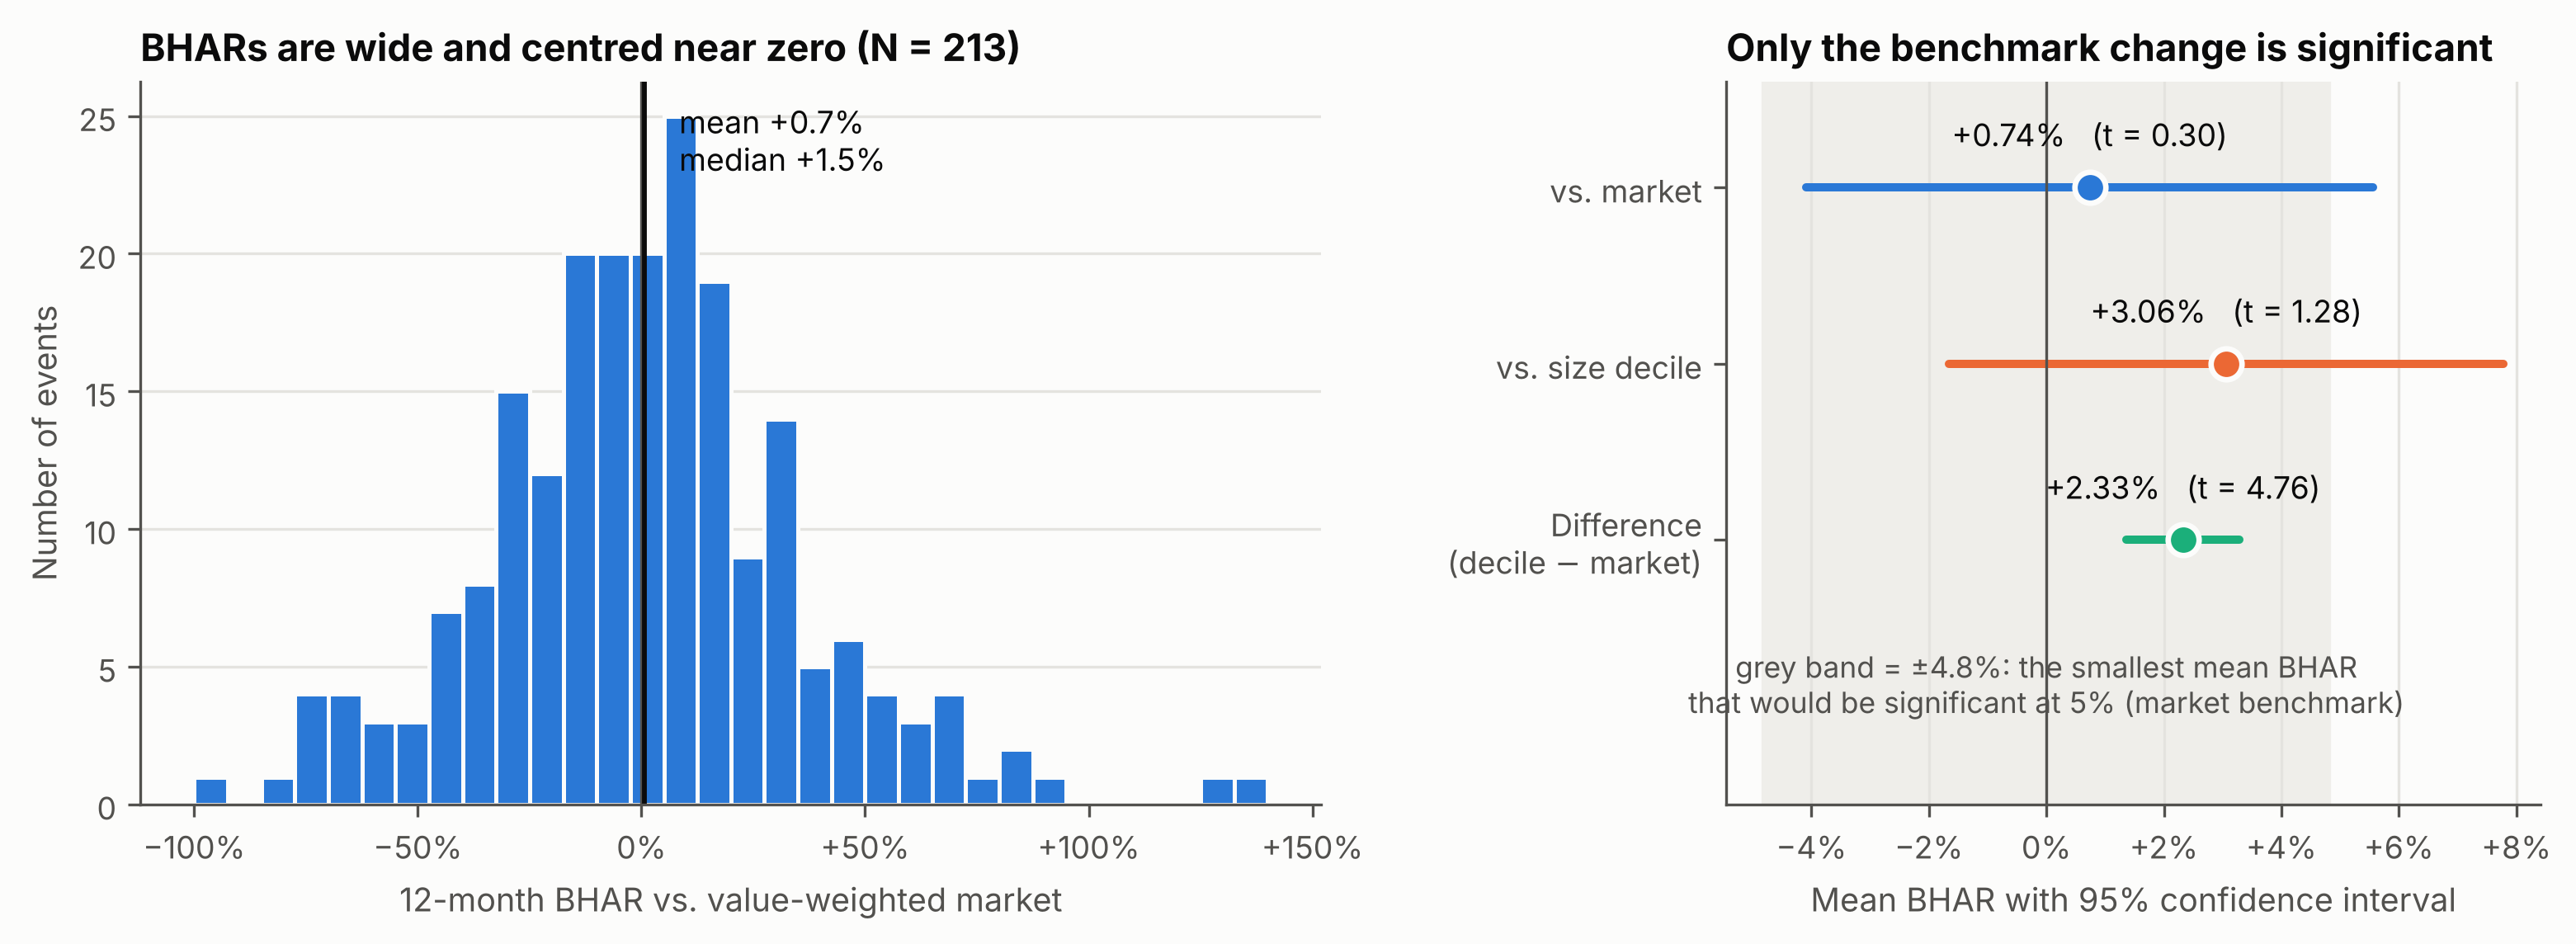
\includegraphics[width=\textwidth]{figures/fig1_bhar.png}
\caption{Q2--Q4. Left: histogram of the 213 12-month BHARs against the value-weighted market (\texttt{mkt\_ret}); the vertical line is the mean (+0.74\%; median +1.53\%). Right: mean BHAR with 95\% confidence intervals for the market benchmark, the size-decile benchmark and their paired difference. The grey band is $\pm4.8\%$, the smallest mean BHAR that would be significant at 5\% given the standard error of the market-benchmark BHAR. Only the change of benchmark is statistically distinguishable from zero.}
\label{fig:bhar}
\end{figure}
\begin{figure}[!htbp]
\centering
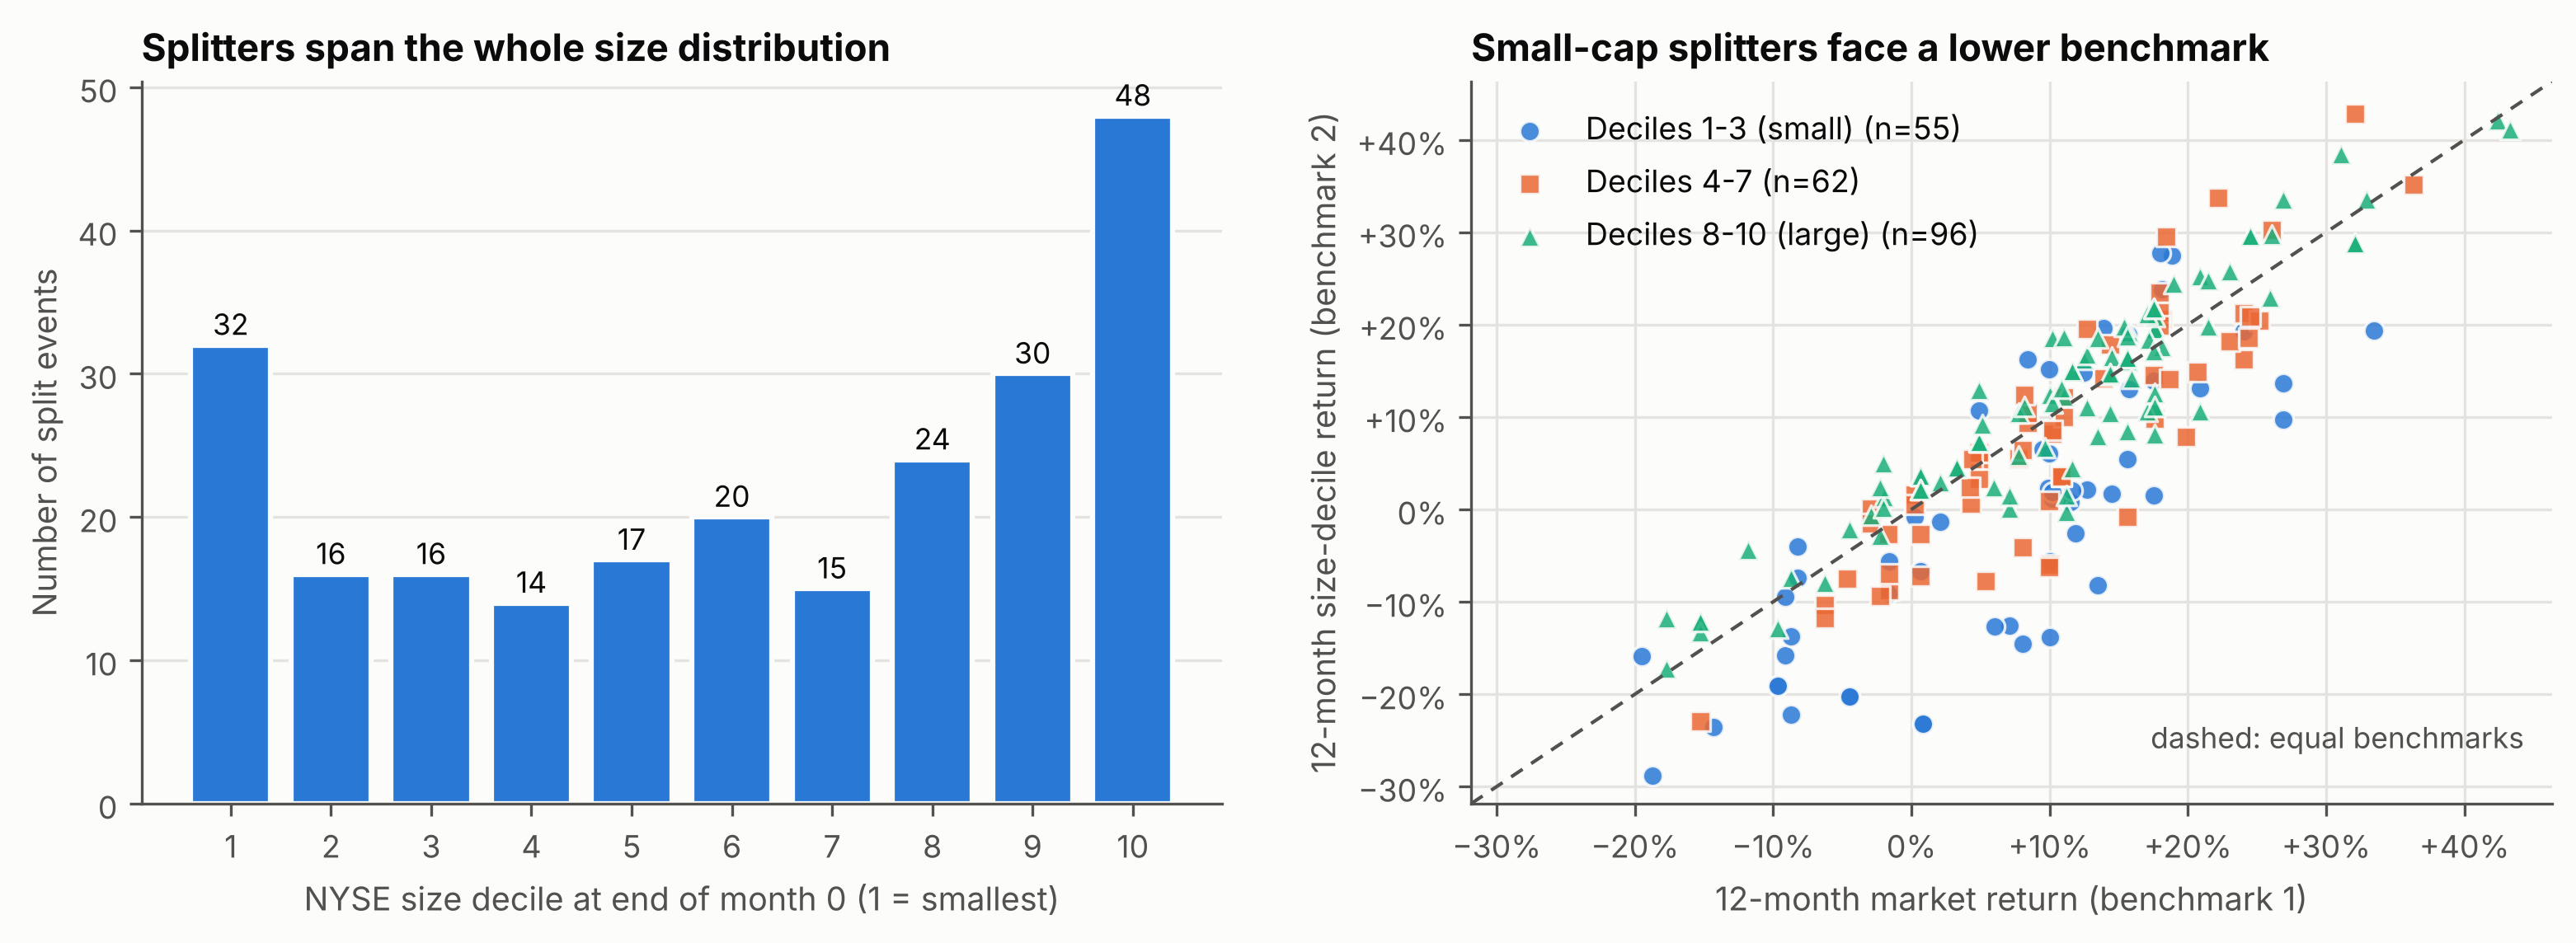
\includegraphics[width=\textwidth]{figures/fig3_size_benchmark.png}
\caption{Q3. Left: number of split events by NYSE size decile (month-0 market cap against French's ME breakpoints). Right: each event's 12-month market return against its size-decile return, by size group; points below the dashed 45-degree line are events whose size-matched benchmark is lower than the market, which is the case for most small-cap splitters.}
\label{fig:size}
\end{figure}
\begin{table}
\caption{Q3 (check): number of split events by NYSE size decile, assigned with market cap at the end of month 0 and French's NYSE ME breakpoints for that month (cap in $ thousands divided by 1,000 to match $ millions).}
\label{tab:decile}
\begin{tabular}{lrr}
\toprule
 & Events & Share \\
NYSE size decile (1 = smallest) &  &  \\
\midrule
1 & 32 & 0.138 \\
2 & 16 & 0.069 \\
3 & 16 & 0.069 \\
4 & 14 & 0.060 \\
5 & 17 & 0.073 \\
6 & 20 & 0.086 \\
7 & 15 & 0.065 \\
8 & 24 & 0.103 \\
9 & 30 & 0.129 \\
10 & 48 & 0.207 \\
\bottomrule
\end{tabular}
\end{table}

\begin{table}[!htbp]
\centering
\small
\caption{Q5: equal-weighted calendar-time portfolio of stocks within months +1 to +12 of a split window (a stock with overlapping splits is held once; a stock is dropped after its last trading month).}
\label{tab:q5}
\begin{tabular}{p{9cm}r}
\toprule
 & Value \\
\midrule
Calendar months in portfolio & 143.0000 \\
Average stocks held & 18.6503 \\
Minimum stocks held & 4 \\
Maximum stocks held & 41 \\
Months with fewer than 10 stocks & 22.0000 \\
Months with zero stocks & 0.0000 \\
Mean monthly portfolio return & 0.0094 \\
Std. dev. of monthly portfolio return & 0.0562 \\
\bottomrule
\end{tabular}
\end{table}

\begin{figure}[!htbp]
\centering
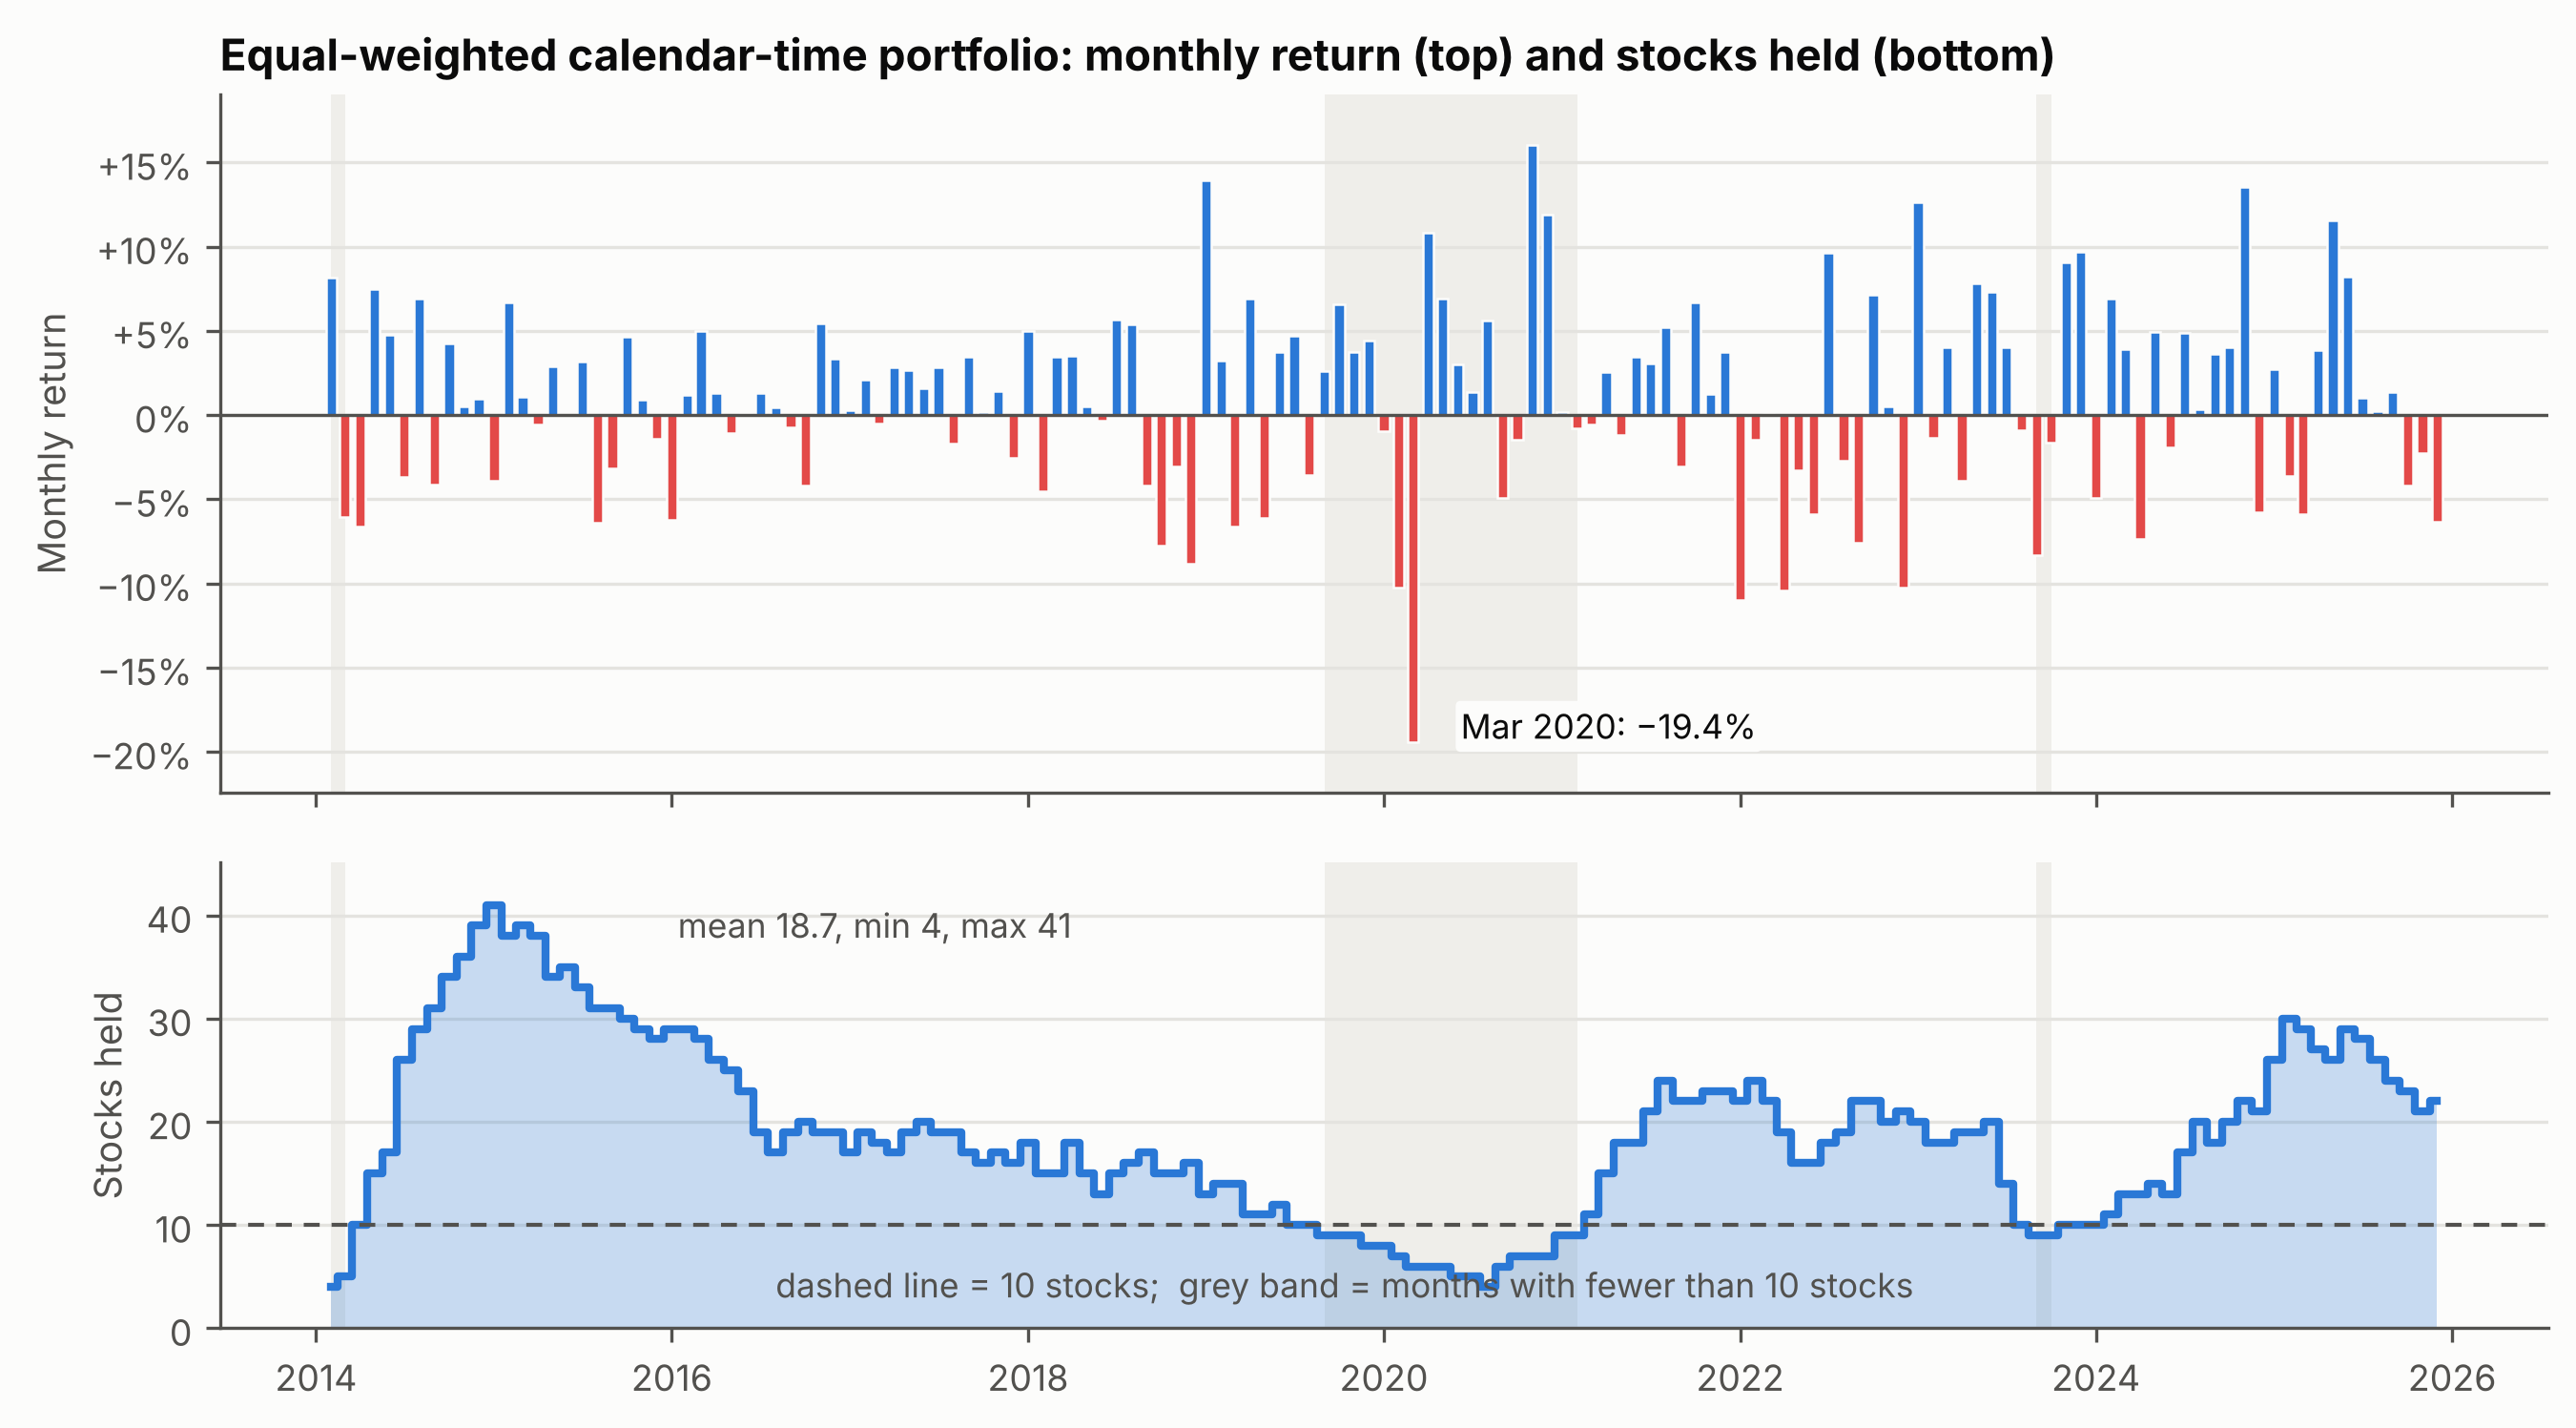
\includegraphics[width=\textwidth]{figures/fig2_portfolio.png}
\caption{Q5. Equal-weighted calendar-time portfolio, Feb 2014--Dec 2025: monthly return in percent (top; blue = gain, red = loss) and number of stocks held (bottom). Grey bands mark the 22 months with fewer than 10 stocks, which are kept in the sample.}
\label{fig:port}
\end{figure}
\begin{table}[!htbp]
\centering
\small
\caption{Q6: regressions of the equal-weighted calendar-time portfolio's monthly excess return ($R_p - R_f$) on factors. Alpha in percent per month; loadings are betas. Model (5) uses the five-factor file's own Mkt-RF, SMB, HML, RMW, CMA and RF. Sample: calendar months with at least one stock held.}
\label{tab:q6}
\begin{tabular}{lrrrrr}
\toprule
 & (1) No factors & (2) CAPM & (3) FF3 & (4) FF3+Mom & (5) FF5 \\
\midrule
\rowcolor[gray]{0.94} \textbf{alpha (\% per month)} & \textbf{0.796\textsuperscript{**}} & \textbf{$-$0.325} & \textbf{$-$0.121} & \textbf{$-$0.124} & \textbf{$-$0.114} \\
\rowcolor[gray]{0.94}  & [2.27] & [$-$1.52] & [$-$0.51] & [$-$0.53] & [$-$0.48] \\
\rowcolor[gray]{0.94}  & (1.70) & ($-$1.29) & ($-$0.53) & ($-$0.54) & ($-$0.49) \\
\addlinespace
Mkt-RF &  & 1.102\textsuperscript{***} & 1.003\textsuperscript{***} & 1.005\textsuperscript{***} & 0.988\textsuperscript{***} \\
 &  & [23.20] & [26.66] & [22.42] & [24.37] \\
\addlinespace
SMB &  &  & 0.505\textsuperscript{***} & 0.507\textsuperscript{***} & 0.456\textsuperscript{***} \\
 &  &  & [7.86] & [7.93] & [6.65] \\
\addlinespace
HML &  &  & $-$0.091 & $-$0.088 & $-$0.114 \\
 &  &  & [$-$1.10] & [$-$0.96] & [$-$0.99] \\
\addlinespace
Mom &  &  &  & 0.009 &  \\
 &  &  &  & [0.11] &  \\
\addlinespace
RMW &  &  &  &  & $-$0.045 \\
 &  &  &  &  & [$-$0.33] \\
\addlinespace
CMA &  &  &  &  & $-$0.151 \\
 &  &  &  &  & [$-$0.92] \\
\midrule
N months & 143 & 143 & 143 & 143 & 143 \\
R-squared & 0.000 & 0.729 & 0.785 & 0.785 & 0.784 \\
SE alpha, OLS (\%) & 0.470 & 0.252 & 0.229 & 0.231 & 0.232 \\
SE alpha, Newey-West (\%) & 0.351 & 0.213 & 0.235 & 0.235 & 0.235 \\
\bottomrule
\end{tabular}
\par\vspace{3pt}
{\footnotesize Stars: significance of the Newey-West $t$ (* 10\%, ** 5\%, *** 1\%). Brackets: Newey-West $t$ (6 lags); parentheses: OLS $t$ (alpha only).}
\end{table}

\begin{figure}[!htbp]
\centering
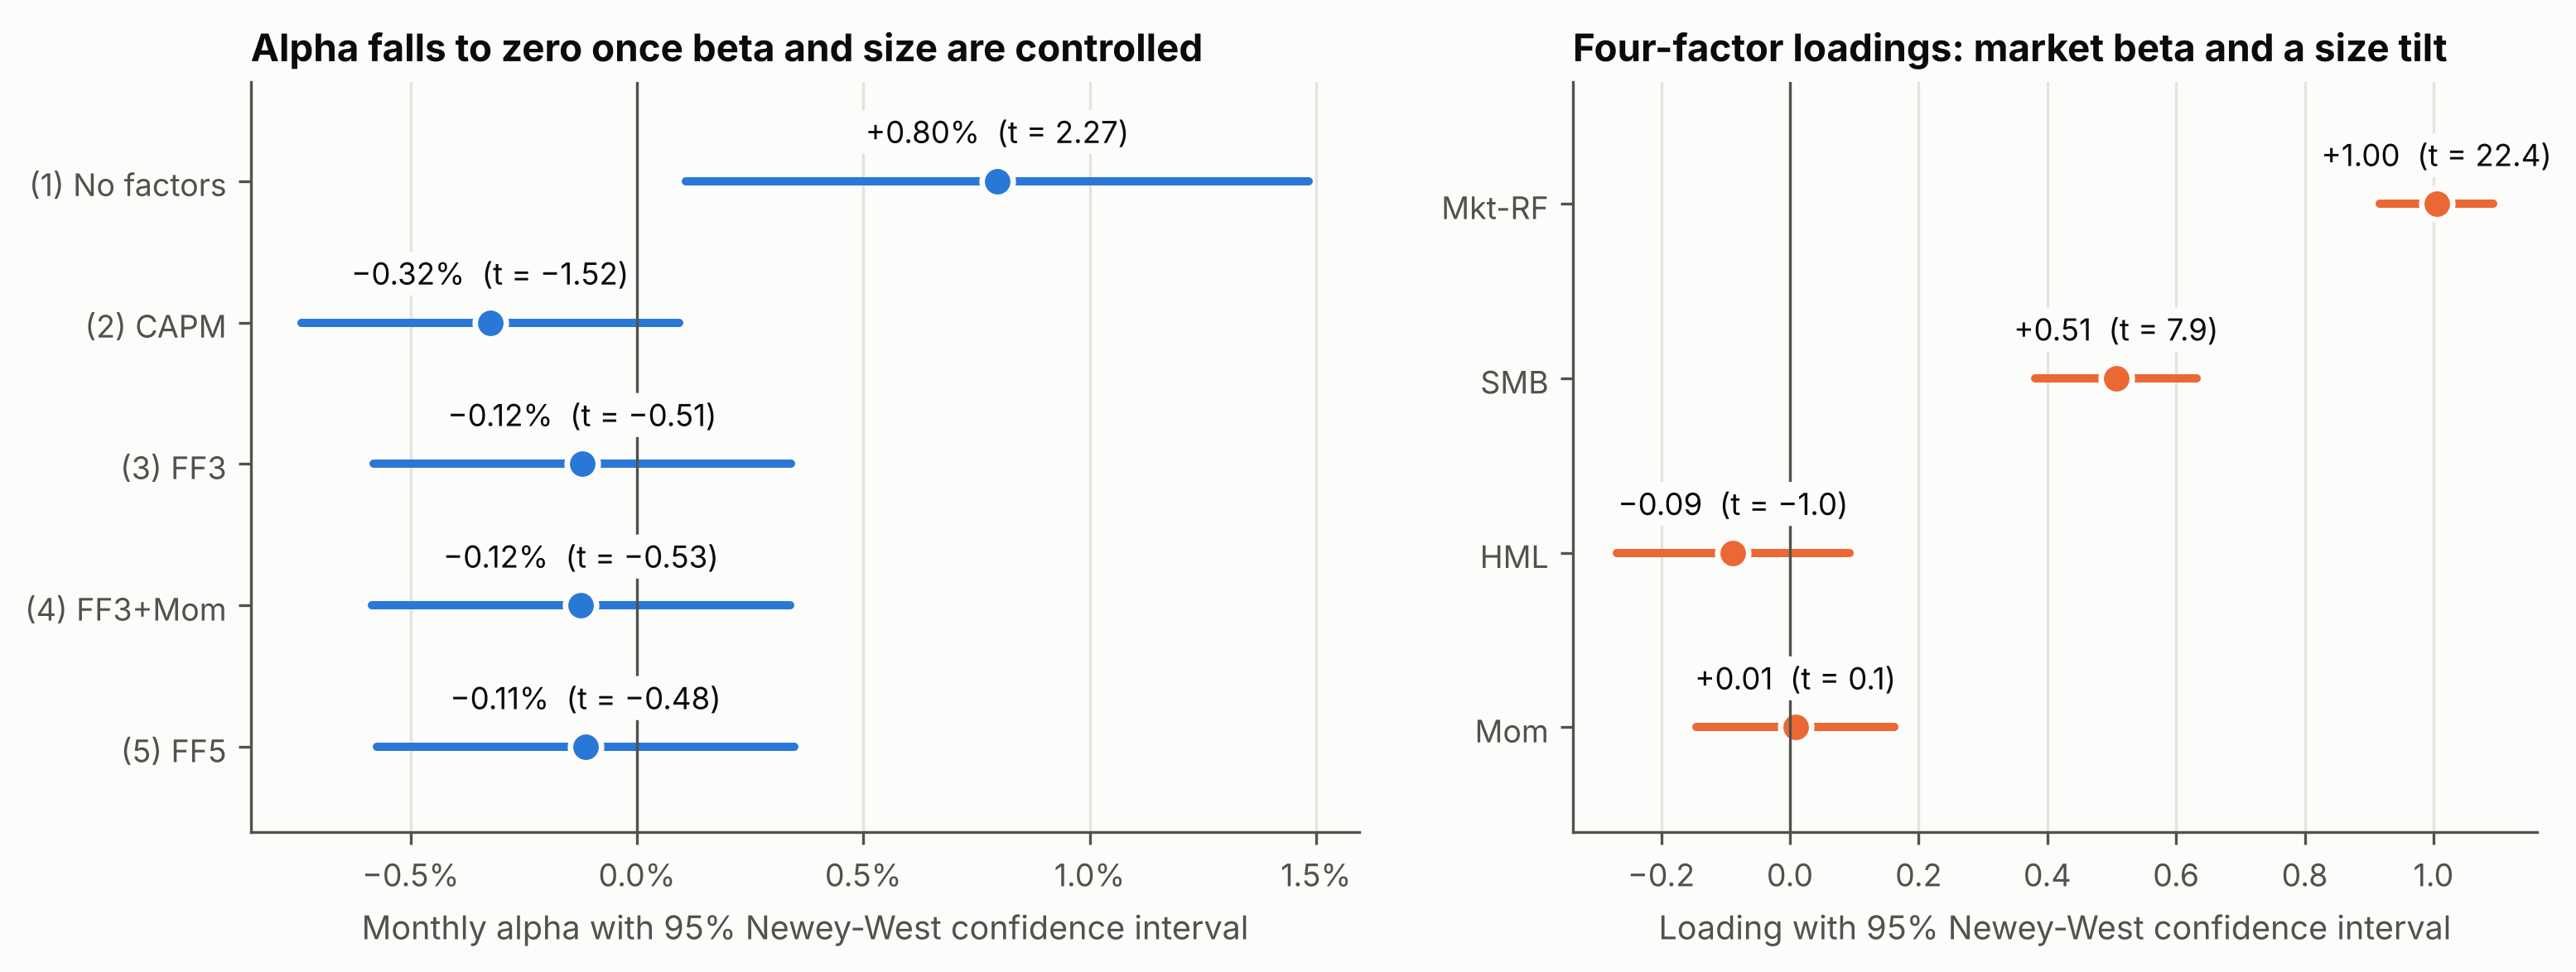
\includegraphics[width=\textwidth]{figures/fig4_alpha_loadings.png}
\caption{Q6. Left: monthly alpha of the portfolio under each model with 95\% Newey-West confidence intervals (labels: alpha and Newey-West $t$). Right: factor loadings of the four-factor model with 95\% confidence intervals. The raw excess return is significant; once the market (beta 1.0--1.1) and size (SMB 0.5) are controlled, alpha is indistinguishable from zero.}
\label{fig:alpha}
\end{figure}
\begin{table}[!htbp]
\centering
\small
\caption{Q6 (robustness): Newey-West $t$-statistic of alpha for different lag lengths (0 lags = White heteroskedasticity-robust). The conclusion does not depend on the lag choice.}
\label{tab:q6b}
\begin{tabular}{lrrrr}
\toprule
 & NW t(alpha), 0 lags & NW t(alpha), 3 lags & NW t(alpha), 6 lags & NW t(alpha), 12 lags \\
\midrule
(2) CAPM & $-$1.34 & $-$1.38 & $-$1.52 & $-$1.83 \\
(3) FF3 & $-$0.56 & $-$0.52 & $-$0.51 & $-$0.56 \\
(4) FF3+Mom & $-$0.56 & $-$0.53 & $-$0.53 & $-$0.57 \\
\bottomrule
\end{tabular}
\end{table}

\begin{table}[!htbp]
\centering
\small
\caption{Q6 (supporting): decomposition of the portfolio's mean monthly excess return (percent per month) into alpha and (loading $\times$ sample-mean factor). The last row equals the first row (identity check). Moving from CAPM to three factors raises alpha by 0.20 pp: 0.10 pp from a lower market beta and 0.11 pp from the SMB loading times the negative SMB premium.}
\label{tab:q6c}
\begin{tabular}{lrrrr}
\toprule
 & (2) CAPM & (3) FF3 & (4) FF3+Mom & (5) FF5 \\
\midrule
Mean excess return (\%/month) & 0.796 & 0.796 & 0.796 & 0.796 \\
\rowcolor[gray]{0.94} \textbf{Alpha} & \textbf{$-$0.325} & \textbf{$-$0.121} & \textbf{$-$0.124} & \textbf{$-$0.114} \\
\addlinespace
Mkt-RF: loading x mean factor & 1.121 & 1.019 & 1.021 & 1.005 \\
SMB: loading x mean factor &  & $-$0.112 & $-$0.112 & $-$0.111 \\
HML: loading x mean factor &  & 0.009 & 0.009 & 0.012 \\
Mom: loading x mean factor &  &  & 0.001 &  \\
RMW: loading x mean factor &  &  &  & $-$0.013 \\
CMA: loading x mean factor &  &  &  & 0.017 \\
\midrule
Sum (alpha + contributions) & 0.796 & 0.796 & 0.796 & 0.796 \\
\bottomrule
\end{tabular}
\end{table}

\begin{table}
\caption{Q6 (supporting): mean and standard deviation of the factors over the portfolio's months (percent per month).}
\label{tab:q6d}
\begin{tabular}{lrr}
\toprule
 & Mean (\%/month) & Std. dev. (\%/month) \\
\midrule
Mkt-RF & 1.017 & 4.349 \\
SMB & -0.221 & 2.752 \\
HML & -0.103 & 3.620 \\
Mom & 0.163 & 3.822 \\
RMW\_5 & 0.286 & 2.086 \\
CMA\_5 & -0.110 & 2.287 \\
\bottomrule
\end{tabular}
\end{table}

\begin{table}[!htbp]
\centering
\small
\caption{Q7 (bridge): from the 12-month BHAR to the calendar-time alphas, in percent per year. (a)-(b) change only the benchmark; (c)-(d) change from event weighting to calendar-month weighting and from compounded to arithmetic returns; (f)-(h) let the model adjust for market beta and style loadings. Alphas are monthly alphas multiplied by 12. French market = Mkt-RF + RF.}
\label{tab:q7}
\begin{tabular}{p{9cm}r}
\toprule
 & Percent per year \\
\midrule
\rowcolor[gray]{0.94} \textbf{(a) Mean 12-month BHAR vs. mkt\_ret} & \textbf{0.74} \\
(b) Mean 12-month BHAR vs. French market & $-$0.62 \\
\addlinespace
(c) Event-month mean of (R\_i - mkt\_ret) x 12 & 0.93 \\
(d) Calendar-month mean of (R\_p - mkt\_ret) x 12 & $-$1.35 \\
(e) Calendar-month mean of (R\_p - French market) x 12 & $-$2.65 \\
\addlinespace
\rowcolor[gray]{0.94} \textbf{(f) CAPM alpha x 12} & \textbf{$-$3.89} \\
(g) Three-factor alpha x 12 & $-$1.45 \\
(h) Four-factor (with Mom) alpha x 12 & $-$1.49 \\
\bottomrule
\end{tabular}
\end{table}

\begin{figure}[!htbp]
\centering
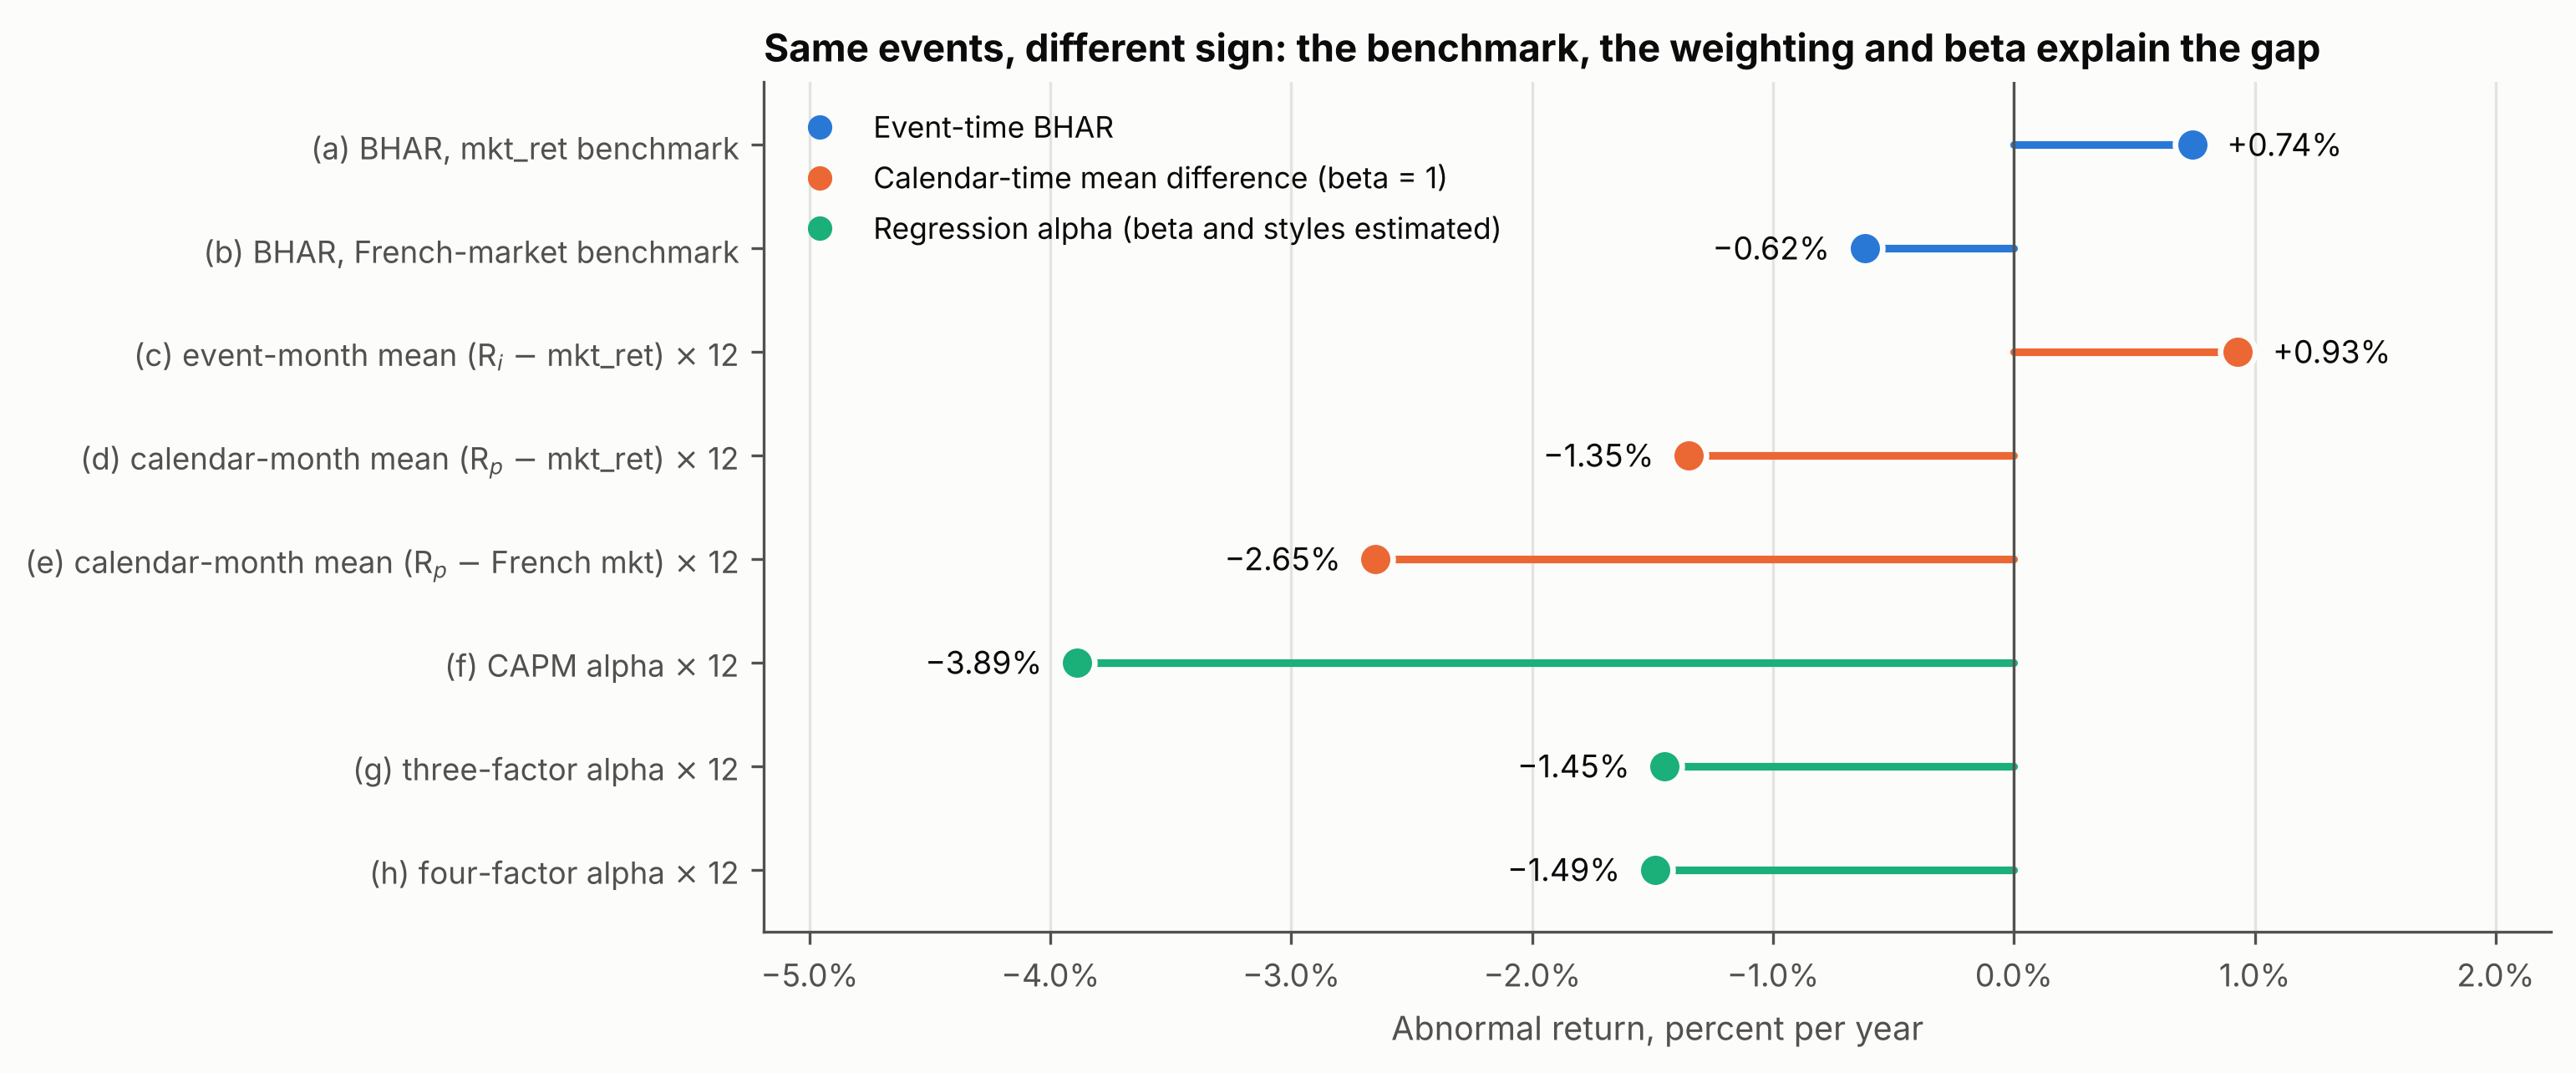
\includegraphics[width=0.9\textwidth]{figures/fig5_bridge.png}
\caption{Q7. From the 12-month BHAR to the calendar-time alphas, in percent per year (same split events throughout). Blue: event-time BHAR; orange: mean difference between the calendar-time portfolio and the market (beta fixed at one); green: regression alphas (monthly alpha $\times$ 12). The point estimates change sign because of the benchmark, the weighting and the estimated beta; none is statistically significant.}
\label{fig:bridge}
\end{figure}
\begin{table}[!htbp]
\centering
\small
\caption{Q8: monthly alpha (percent) by weighting scheme. Equal-weighted: the Q6 portfolio, OLS across months. WLS: same portfolio, each month weighted by the number of stocks held. Value-weighted: stocks weighted by market cap at the end of the previous month, OLS across months.}
\label{tab:q8}
\begin{tabular}{lrrrrrr}
\toprule
 & \multicolumn{2}{c}{Equal-weighted, OLS} & \multicolumn{2}{c}{Equal-weighted, WLS (w = N)} & \multicolumn{2}{c}{Value-weighted, OLS} \\
\cmidrule(lr){2-3}\cmidrule(lr){4-5}\cmidrule(lr){6-7}
 & alpha (\%) & t (NW) & alpha (\%)  & t (NW)  & alpha (\%)   & t (NW)   \\
\midrule
(1) No factors & 0.796\textsuperscript{**} & [2.27] & 0.710\textsuperscript{**} & [2.12] & 1.215\textsuperscript{**} & [2.37] \\
(2) CAPM & $-$0.325 & [$-$1.52] & $-$0.176 & [$-$0.80] & $-$0.065 & [$-$0.16] \\
(3) FF3 & $-$0.121 & [$-$0.51] & 0.036 & [0.15] & $-$0.147 & [$-$0.41] \\
(4) FF3+Mom & $-$0.124 & [$-$0.53] & 0.024 & [0.10] & $-$0.104 & [$-$0.29] \\
(5) FF5 & $-$0.114 & [$-$0.48] & 0.029 & [0.12] & $-$0.165 & [$-$0.50] \\
\bottomrule
\end{tabular}
\par\vspace{3pt}
{\footnotesize Stars: significance of the Newey-West $t$ (6 lags, in brackets): * 10\%, ** 5\%, *** 1\%. Usual OLS $t$-statistics are in table8\_weighting\_full.csv and give the same conclusions.}
\end{table}

\begin{figure}[!htbp]
\centering
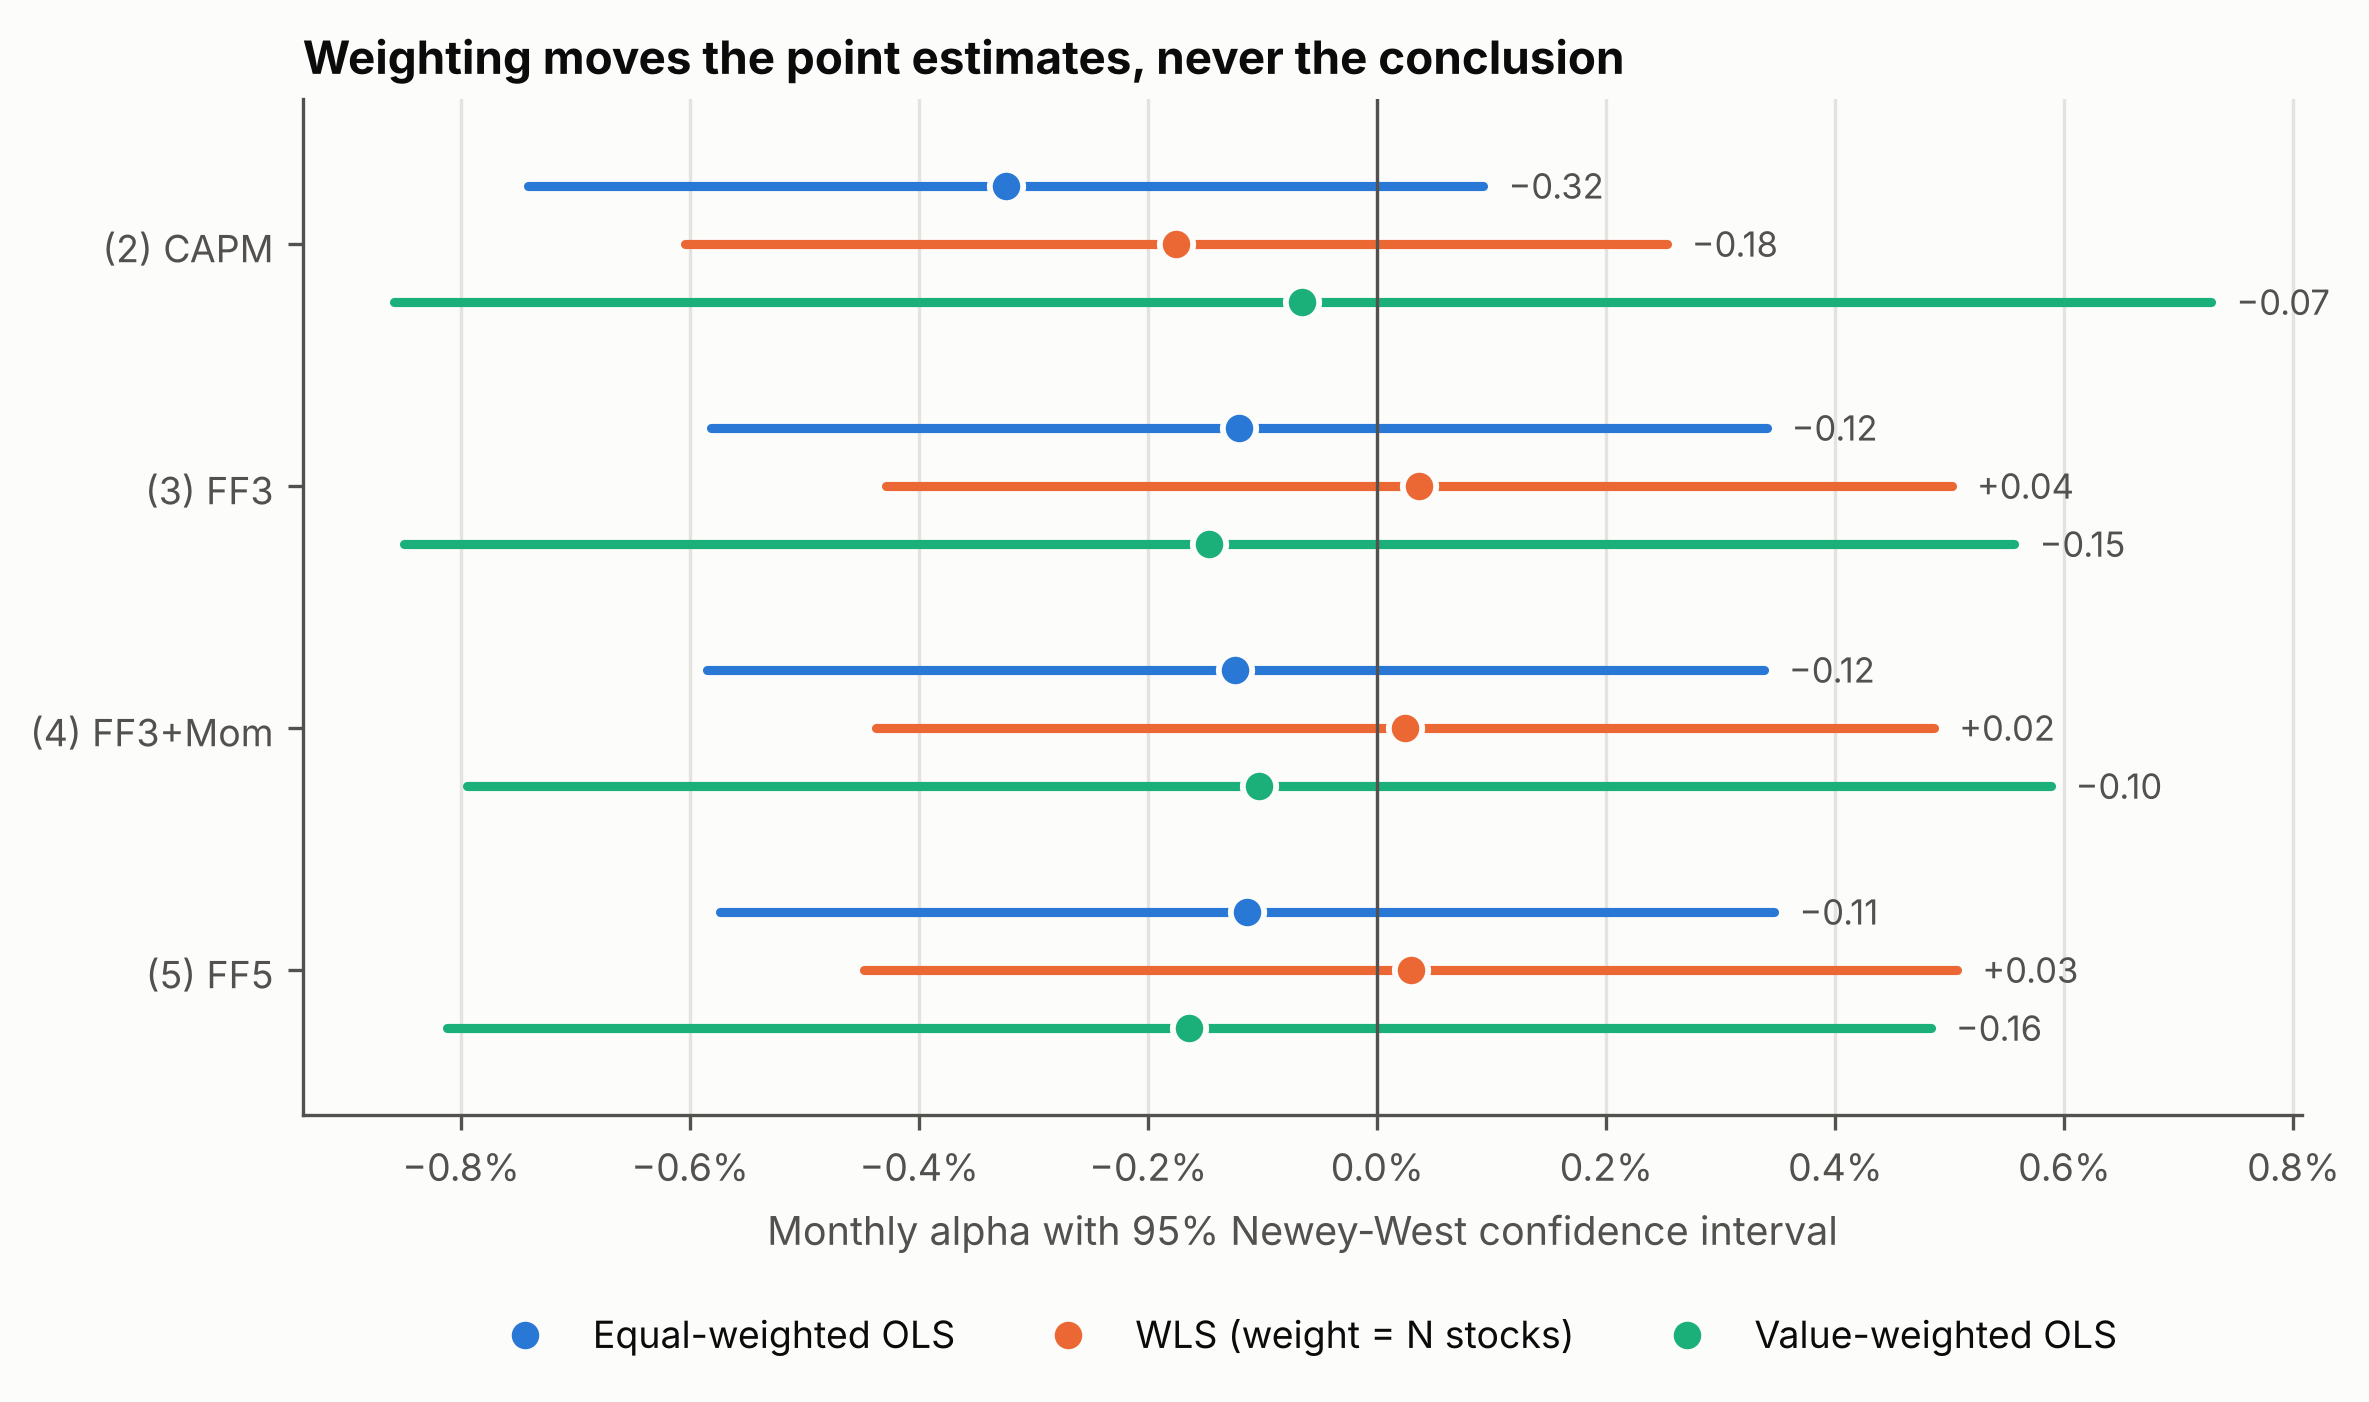
\includegraphics[width=0.9\textwidth]{figures/fig6_weighting.png}
\caption{Q8. Monthly alpha by weighting scheme and model (without the no-factor model, whose alpha is the raw mean return), with 95\% Newey-West confidence intervals. All intervals contain zero; value-weighted intervals are widest because the portfolio holds about four effective stocks.}
\label{fig:weight}
\end{figure}
\begin{table}[!htbp]
\centering
\small
\caption{Q8 (supporting): factor loadings under each weighting scheme. The value-weighted portfolio is a large-cap growth portfolio (beta 1.2--1.3, HML $\approx -0.75$, SMB $\approx 0$).}
\label{tab:q8b}
\begin{tabular}{lrrrr}
\toprule
 & Mkt-RF & SMB & HML & Mom \\
\midrule
EW (3) FF3 & 1.003 & 0.505 & $-$0.091 &  \\
EW (4) FF3+Mom & 1.005 & 0.507 & $-$0.088 & 0.009 \\
WLS (3) FF3 & 0.981 & 0.465 & $-$0.130 &  \\
WLS (4) FF3+Mom & 0.988 & 0.471 & $-$0.121 & 0.028 \\
VW (3) FF3 & 1.260 & $-$0.013 & $-$0.749 &  \\
VW (4) FF3+Mom & 1.227 & $-$0.048 & $-$0.791 & $-$0.128 \\
\bottomrule
\end{tabular}
\end{table}


\clearpage
\section*{Appendix: Data checks and judgment note}

\noindent\textbf{Checks.} The unit of observation is the event-month (event panel: 230 events, 2,681 rows) for Q1--Q4 and the calendar month (143 months) for Q6--Q8. Table~\ref{tab:checks} reports the main checks. The raw data have no duplicates and no missing values (629,274 stock-days, 202 stocks, 232 events, all with data in month 0). The empty returns are 91 missing stock-days inside a stock's history (0.015\% of stock-days), filled with the market return; only 2 events contain a filled day. Another 923 missing stock-days fall in months where the stock has no data at all; these months are treated as ``stopped trading'' (4 events). Panel rows equal the expected number, and BHARs recomputed directly from daily data agree to $10^{-15}$. Monthly market returns correlate 0.998 with French's market but are about 0.11 pp per month lower. Units: \texttt{mktcap} in \$ thousands is divided by 1,000 to match French's breakpoints in \$ millions; French returns are divided by 100; alphas are shown in percent per month. Equal and value weights sum to one in every month; the CAPM and mean-return regressions match closed-form OLS; the alpha decomposition identity holds. Magnitudes look right: monthly market return mean 1.1\%, sd 4.1\%; 143 of 143 months have at least one stock; the portfolio's monthly return range is $-19.4$\% to $+16.0$\%.

\medskip
\noindent\textbf{Judgment.} (1) \emph{Benchmark.} The provided \texttt{mkt\_ret} is not French's market (about 1.4 pp per year lower), and I used it for BHAR as instructed. Against French's market the mean BHAR is $-0.6$\% ($t=-0.26$), so the sign of the BHAR depends on this choice, but not its insignificance. (2) \emph{Size deciles and gaps.} Decile benchmarks use month-0 cap with that month's NYSE breakpoints, whereas French's decile portfolios are reformed each June; a firm that moves across deciles within the year is benchmarked to a portfolio whose composition differs from its own. Events cluster in time (iid s.e.\ 2.44\% against 2.37\% clustered by ex-date month), and the 12-month windows overlap, so t-statistics may be overstated; Newey-West with 6 lags handles part of this in the calendar-time regressions. The fill rule affects only 2 events and the stopped-trading rule 4; excluding them gives a mean BHAR of 0.78\% ($t=0.32$) and a CAPM alpha of $-0.32$\% ($t=-1.47$), and winsorising BHARs at 1/99 gives 0.46\% ($t=0.20$) (Table~\ref{tab:rob}), so no conclusion depends on these rules.

\begin{table}
\caption{Robustness: dropping the events touched by the empty-day fill rule (2) or the stopped-trading rule (4), and winsorising BHARs at the 1st and 99th percentiles. Estimates are percent (BHAR) or percent per month (alpha); t-statistics are conventional for BHAR and Newey-West for alpha.}
\label{tab:rob}
\begin{tabular}{p{8cm}rrr}
\toprule
 & N & Estimate (\%) & t-statistic \\
\midrule
BHAR vs. market, excluding fill/stop events & 208 & 0.780 & 0.320 \\
BHAR vs. market, winsorised at 1/99 & 213 & 0.460 & 0.200 \\
CAPM alpha (\%/month), excluding fill/stop events & 143 & -0.320 & -1.470 \\
\bottomrule
\end{tabular}
\end{table}

\begin{table}[!htbp]
\centering
\small
\caption{Appendix: data and results checks (selected). Full list in sanity\_checks.csv.}
\label{tab:checks}
\begin{tabular}{p{9cm}p{6cm}}
\toprule
 & Result \\
\midrule
daily rows & 629274 \\
split events & 232 \\
daily duplicates (permno,date) & 0 \\
daily missing ret / mkt\_ret / mktcap & 0 / 0 / 0 \\
ex-date range & 2014-01-08 to 2025-12-23 \\
trading days in calendar & 3520 \\
explicit NaN ret in raw file & 0 \\
empty stock-days inside stock history filled with mkt\_ret & 91 \\
stock-days in wholly-empty months (not filled, month treated as 'stopped trading') & 923 \\
corr(compounded mkt\_ret, French Mkt-RF+RF) monthly & 0.99772 \\
mean monthly diff (mkt\_ret - French Mkt), and 2014-2025 compounded return of each & $-$0.00115; 2.825 vs 3.420 \\
events with trading obs in month 0 & 232 of 232 \\
monthly stock return inside event windows: min / max & $-$0.585 / 1.054 \\
expected panel rows = sum(min(12, DATA\_END - m0)) & 2681 \\
BHAR from panel vs direct daily compounding (8 random events), max abs diff & 2.66e-15 \\
events whose window contains a day filled with mkt\_ret & 2 \\
robustness: mean BHAR vs French market / t & $-$0.0062 / $-$0.26 \\
SE of mean BHAR: iid vs clustered by ex-date month & 0.0244 vs 0.0237 \\
events with size decile assigned & 232 of 232 \\
cap at month 0: median / min / max (\$ millions) & 5,324 / 23.4 / 3,035,234 \\
held event-months before / after removing overlapping splits of the same stock & 2675 / 2667 \\
EW weights sum to 1 in every month (max abs deviation) & 0.00e+00 \\
model (1) alpha == mean excess return & 0.007960 vs 0.007960 \\
CAPM alpha/beta: statsmodels vs numpy lstsq (max abs diff) & 2.22e-16 \\
VW weights sum to 1 in every month (max abs deviation) & 2.22e-16 \\
VW: average / max (over months) of largest single-stock weight & 0.502 / 0.944 \\
VW: average effective number of stocks (1/sum w\textasciicircum{}2) & 3.7 \\
decomposition identity: max |sum - mean excess| & 1.4e-14 \\
\bottomrule
\end{tabular}
\end{table}


\end{document}
